\graphicspath{{Ch1_Theory/figures/}}

\chapter{Theoretical Framework}

% HOW TO DO CITATIONS/FIGURES/EQN/REFERENCES

% \cite{Belytschko1994a

% \begin{figure}
% 	\includegraphics[width=0.85\textwidth]{sbm.png}
% 	\caption{SBM}
% 	\label{fig:sbm_fig}
% \end{figure}
% This is how I reference a figure \autoref{fig:sbm_fig}
% 
% \begin{equation}
% a = b + c
% \label{eqn:equation}
% \end{equation}
% I referenced equations like this
% \eqref{eqn:equation}

The Standard Model (SM) of particle physics is the most successful theory in the history of human scientific endeavour.
It provides a unified framework describing the electroweak and strong interactions along with all known particles that participate in those interactions.
The fundamental objects in the SM description are fields defined at all points in spacetime.
The SM fields fall into four main categories:

\nomenclature[A]{SM}{The \textbf{S}tandard \textbf{M}odel of Particle Physics}
\nomenclature[A]{QFT}{\textbf{Q}uantum \textbf{F}ield \textbf{T}heory}

\begin{enumerate}
    \item Fermionic fields, $\psi$, describing ``matter'': quarks and leptons
    \item Electroweak Spin-1 Boson fields
        \begin{itemize}
            \item $W_1, W_2, W_3, B$: before symmetry breaking
            \item $W^+, W^-, Z^0, \gamma$: after symmetry breaking
        \end{itemize}
    \item Gluon fields, $G_a$.
    \item The Higgs field, $\varphi$.
\end{enumerate}

The dynamics of these fields are predicted via the mathematical framework of Quantum Field Theory (QFT).
%, or more specifically, quantum Yang-Mills gauge theories with certain symmetries imposed upon the Lagrangian density $\mathcal{L}$.
The historical path taken to arrive at the Standard Model is a winding one indeed.
In this chapter a brief but complete overview of the mathematical framework of the Standard Model is given, but divorced from historical order of development, in order to explain what the Standard Model \textit{is} rather than \textit{how} it came to be.

\begin{figure}[h]
   \centering
    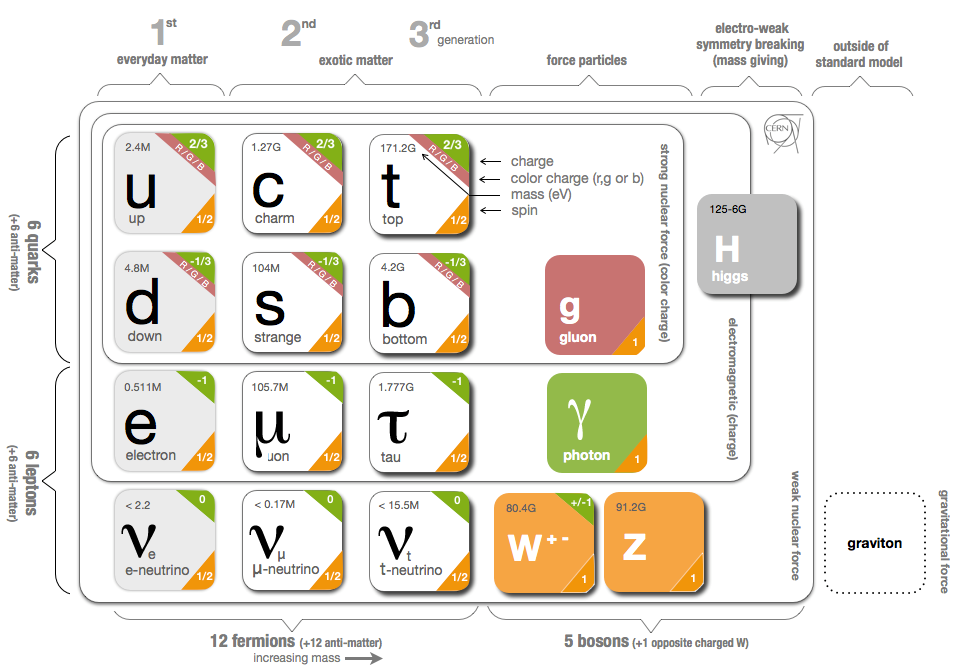
\includegraphics[width=\textwidth]{SMdiagram}
    \caption{Phenomenological breakdown of the Standard Model. © 2014 CERN}
\end{figure}

\section{Symmetry}
% The arena in which all particles are embedded in the Standard Model is the pseudo-Riemannian manifold $\mathbb{R}^{3,1}$, otherwise known as Minkowski space.
% More explicitely, $\mathbb{R}^{3,1}$ is the gathering of Euclidean three-dimensional space and time into a four-dimensional manifold equipped with a non-degenerate,
% symmetric binlinear form $\eta_{\mu\nu}$ on the tangent space at each point in spacetime, often referred to as the \textit{Minkowski metric}.
% The spacetime interval between two arbitrary elements of the tangent space, $x$ and $y$, is given by $s^2 \equiv \myavg{x,y} = \eta_{\mu\nu}x^\mu y^\nu$.
% The isometry group of $\mathbb{R}^{3,1}$ (i.e. the set of all bijective $s^2$-preserving maps from $\mathbb{R}^{3,1}$ to $\mathbb{R}^{3,1}$) is known as the Poincar\'{e} group.
% 
% Particles have additional internal properties which must be described in a spacetime independent way. This means that the symmetry group of the universe must actually be described by the \textit{direct product} of two groups, one encapsulating the properties of spacetime itself, and the other encoding the internal degrees of freedom of the particles embedded in this spacetime.
% The internal symmetry group of the standard model is $SU(3)_C, \times SU(2)_L \times U(1)_Y$, the meaning of which is elaborated on below.
% 
\section{Fields}
% A central assumption of the Standard Model, motivated by many different experimental and theoretical results, is that the laws of physics are invariant with respect to Poincar\'{e} transformations: elements of the Poincar\'{e} group.
% Thus in order to describe particles, representations of the Poincar\`{e} group must be used.
% Following from work of Eugene Wigner [NEEDREF], all the mathematical structures (fields) used to describe particles in the Standard Model are positive-energy irreducible unitary representation of the Poincar\'{e} group.
% The Lorentz group is \textit{semisimple} and can be written as
% 
% \begin{equation}
%     so(1,3) = su(2) \oplus su(2)
% \end{equation}
% 
% which means that all representations of the Lorentz group so(1,3) can be built up as direct sums of representations of su(2).
% Each representatino of su(2) can be classified by a half integer $j = 0,1/2,1,3/2,\dots$, which means that each representation of so(1,3) can be classified by a pair of half integers $(n,m)$.
% 
% 
\section{Gauge Invariance}
% A \textbf{gauge} is a choice of spacetime varying coordinate system for the internal symmetry group.
% A \textbf{gauge transformation} is a simultaneous change of this coordinate system at all points in spacetime.
% A \textbf{gauge theory} is a physical model to which gauge transformations can be applied, but with the important caveat that the \textit{physical predictions remain the same} regardless of which gauge is used.
% 
% The necessity for the concept of gauge invariance is due to the presence of mathematical \textit{redundancy} in the degrees of freedom of fields in a gauge theory.
% For example, consider a single particle quantum mechanical system with Hilbert space $H$ and energy eigenstates $\ket{n}$.
% To make a physical prediction for the probability for state $\ket{n}$ at time $t_0$ to evolve into state $\ket{n^\prime}$ at time $t$, one calculates the transition probability $\myabs{\braket{n^\prime(t)|n(t_0)}}^2$.
% However, if one were to make the change of basis $\ket{n} \rightarrow e^{i\theta_n} \ket{n}$, the probability would not change.
% 
% In this sense, the computations are performed in $H$, while the physical states themselves lie in $P(H)$, the \textit{projective} Hilbert space.
% This projective Hilbert space contains set of all equivalence classes of states where $\ket{n} \sim e^{i\theta_n}\ket{n}$, for all $\theta_n$.
% This should not be taken to mean that the redundant degrees of freedom in a gauge theory (like the complex phase factor above) are meaningless. 
% While they are not themselves measurable, their presence in the theory has measurable \textit{consequences}.
% For example, the presence of complex phase factors in QM is what leads to the double slit and Ahranov-Bohm effect.
% These consequence arise from the \textit{difference} in phase factors between states that naturally arise througout the calculation, but do not depend on the initial choices of $\theta_n$.
% 
% In short, the necessity for gauge invariance is that the mathematical/computational framework of a theory may have its \textit{own} internal machinery which contributes to the result but drop out in the final physical prediction.
% Once we include any purely computational degrees of freedom in our theory we must demand that our theory is invariant with respect to the most general possible change in them that does not alter the physical prediction.
% In the words of Murray Gell-Mann, ``Everything not forbidden is compulsory'', a sentiment at the heart of modern physics.
% To state it another way: any arbitrary element of a theory must be treated as \textit{maximally} arbitrary in order to preserve its integrity.
% 
% One aspect left out of the discussion of one-particle systems above is the notion of comparing the gauge at different points in spacetime.
% Suppose you have two vectors $A,B \in R^n$. In order to compare vector $A$ to vector $B$, vector $A$ must be \textit{transported} so that the tails of $A$ and $B$ are located at the same point.
% Furthermore, this transport must be done while keeping $A$ \textit{parallel} to its original direction in order to preserve geometric information such as the relative angle betwen $A$ and $B$.
% The reason this works and is intuitive is that $R^n$ is a flat space (i.e. has no curvature).
% 
% \newcommand{\conn}{ \ensuremath{ \boldsymbol{\mathcal{A}} } }
% However, if one is operating in a space with curvature (or on a field with spacetime varying coordinate system for the internal symmetry group), the notion of \textbf{parallel transport} must be refined.
% What is needed then is not just a measure of the change in a field, but a measure of the change in a field \textit{relative} to the change that occurs purely to the variations in the coordinate system itself.
% The \textbf{covariant derivative} $D_\mu(x) \equiv \partial_\mu + \conn_\mu(x)$ achieves precisely this.
% The extra spacetime-dependent term $\conn_\mu(x)$ that encodes the effect of the varying coordinate system is known as the \textbf{connection}.
% 
% In the case of a quantum field theory with an internal symmetry (Lie) group $G$, the connection is an element of the corresponding Lie Algebra $\mathfrak{g}$, i.e. the infinitesimal generators $T_a$ of $G$.
% In the case of $\mathfrak{su}(n)$, there are $n^2-1$ independent generators. 
% The fact that the connection is an \textit{infinitesimal} transformation is due to the fact that changes in the spacetime varying coordinate system are demanded to be continuous.
% Thus $\conn_\mu$ can be expanded as $\conn_\mu \equiv A_\mu^a T_a$, where the $n^2-1$ different $A_\mu^a$ terms transform under the adjoint representatino of the internal symmetry group.
% In physics it is common notational practice to define $D_\mu \equiv \partial_\mu - igA_\mu^aT_a$, where $g$ is a dimensionless \textit{coupling constant}.
% The $A_\mu^a$ terms are referred to as \textit{connection coefficients}.
% In fact these connection coefficients will turn out to be the fields for the ``force-carrying'' spin-1 gauge bosons of the Standard Model.
% Precisely \textit{why} a spin-1 boson should show up as a connection coefficient in this manner is an puzzling question without a straight-forward answer at the time of writing.
% 
% \begin{remark}
% notation. Greek letters $\mu,\nu,\dots$ will be used to index Minkowski space, and alphabetic characters $a,b,\dots$ will be used to index the Lie algebra generator basis.
% Einstein summation notation is assumed throughout.
% \end{remark}
% 
% With the covariant derivative we can construct the \textbf{curvature form} $F_{\mu\nu} \equiv \frac{1}{g} \comm{D_\mu}{D_\nu}$.
% A simplified picture of the curvature is that it encodes the \textit{strength} and geometric properties of the gauge field $A_\mu$ at a specific point in spacetime.
% For this reason, the curvature is usually referred to as the \textbf{field strength tensor} in physics.
% 
\section{Yang-Mills Theory}
% The starting point for constructing the Standard Model is Yang-Mills gauge theory, which finds its fullest and most beautiful expression in the language of differential geometry.
% In the case of the Standard Model, we can dispense with some of the abstract notions of differential geometry and restrict our attention to theories taking place in Minkowski Space.
% 
% The previous expression give for the curvature can be expanded as
% \begin{align}
%     F_{\mu\nu} &= \partial_\mu \conn_\nu - \partial_\nu \conn_\mu + ig\comm{\conn_\mu}{\conn_\nu}\\
%     &= \partial_\mu A_\nu^aT_a - \partial_\nu A_\mu^aT_a + ig\comm{A_\mu^aT_a}{A_\nu^bT_b}\\
%     \implies F_{\mu\nu}^a &= \partial_\mu A_\nu^a - \partial_\nu A_\mu^a + igf^a_{\ bc}A_\mu^bA_\nu^c
% \end{align}
% where $f_{abc} \equiv $ are the \textbf{structure constants} of the associated Lie algebra.
% 
% In this system of notation, the \textbf{Yang-Mills Action} can be written
% \newcommand{\YML}{ \ensuremath{ \mathcal{L}_\mathrm{YM} } }
% \begin{align}
%     S_{\mathrm{YM}} &= \int d^4x\ \YML\\
%     \mathrm{where}\ \YML &= -\frac{1}{4} F_{\mu\nu}^aF^{\mu\nu}_a
% \end{align}
% which is manifestly both Poincar\'{e} and gauge invariant. It is important to recognize that two bilinear forms are involved in the above expression, one acting over Lie algebra indices and one over Minkowski space indices.
% 
% A Yang-Mills theory can be expanded by embedding more fields into Minkowski space
% \newcommand{\YM}{ \ensuremath{ \mathcal{L}_m\left[ \left\{ \boldsymbol\Psi \right\}, \left\{ D_\mu \boldsymbol\Psi \right\} \right] }}
% \begin{equation}
%     \mathcal{L} = \YM + \YML
% \end{equation}
% where $\left\{ \boldsymbol\Psi \right\}$ is some set of new ``matter fields'' which transform under the fundamental representation of the internal symmetry group.
% The entire $\mathcal{L}_m$ term must be Poincar\'{e} and gauge invariant, which can be achived by judicious use of bilinear covariants and substitution of the standard spacetime derivative $\partial_\mu$ with the covariant derivative $D_\mu$.
% 
% \subsection{$U(1)$}
% The \textbf{circle group} $U(1)$ is abelian and its corresponding Lie Algebra is just the real numbers. It follows that $f^a_{\ bc} = 0$ and 
% $F_{\mu\nu} = \partial_\mu A_\nu - \partial_\nu A_\mu$, with only a single connection coefficient $A_\mu(x)$.
% Utilizing the Dirac Lagrangian we construct a new Lagrangian for $N$ fermions coupled to the $U(1)$ gauge field.
% \begin{equation}
%     \mathcal{L} = \sum_{j=1}^{N} \bar{\psi}_j \left( i\gamma^\mu D_\mu - m \right) \psi_j - \frac{1}{4}F_{\mu\nu}F^{\mu\nu}
% \end{equation}
% which is the familiar Lagrangian of QED where $A_\mu$ is the photon field and $\psi_j$ are the charged fermion fields.
% Of importance is that any coupling between the different fermions would break gauge invariance and is not allowed.
% Thus in order to explain radioactive decay, for example, this $U(1)$ symmetry group must clearly be expanded.
%\subsection{$SU(2)$}
% The \textbf{special unitary} group $SU(2)$ is non-abelian, so the structure constants in the expression for $F_{\mu\nu}$ do not vanish.
% The generators of $SU(2)$ are $t_a \equiv -\frac{i}{2}\sigma_a$, where $\sigma_a$ are the \textit{Pauli matrices}, and $f^a_{\ bc} = \epsilon^a_{\ bc}$, the Levi-Civita symbol (\textbf{not} the Levi-Civita \textit{tensor}).
% In the fundamental representation of $SU(2)$ we now have $N$ fermion doublets $\Psi_j = \left( \psi_1^{(j)} , \psi_2^{(j)} \right)$.
% \begin{equation}
%     \mathcal{L} = \sum_{j=1}^{N} \bar{\Psi}_j \left( i\gamma^\mu D_\mu - m \right) \Psi_j^T - \frac{1}{4}W^a_{\mu\nu}W^{\mu\nu}_a
% \end{equation}
% which couples $\psi_1^{(j)}$ to $\psi_2^{(j)}$ via the $i \bar{\Psi}_j \gamma^\mu D_\mu \Psi_j^T$ term.
% This could represent, for example, a coupling between electrons $\psi_1$ and electron anti-neutrinos $\psi_2$. 
% There are a few major problem with this idea.
% The most immediate of which is that if $\psi_1$ and $\psi_2$ have different masses,
% splitting the mass term up as $\Psi_j \bigl(\begin{smallmatrix} m_1&0 \\ 0&m_2 \end{smallmatrix}\bigr) \Psi_j^T$ is not gauge invariant.
% 
% \subsection{$SU(2) \times U(1)$}
% \subsection{$SU(3)$}
% \subsection{$SU(3)_c \times SU(2)_L \times U(1)_Y$}
\section{Electroweak Symmetry Breaking}
\section{Renormalization}
\section{Beyond the Standard Model}

\section{Monte Carlo Simulation}

\subsection{Event Generation}

\subsection{Parton Showering}

\subsection{Hadronization}

\subsection{Underlying Event}

\subsection{Tunes}

\subsection{Detector Simulation}
% 